\documentclass{article}

\usepackage{amsmath, mathrsfs, amssymb, stmaryrd, cancel, relsize,tikz,amsthm,comment,graphicx}

\theoremstyle{definition}
\newtheorem{Q}{Question}

\newcommand{\tvs}{\textvisiblespace}
\newcommand{\ra}{\rightarrow}
\newcommand{\la}{\leftarrow}
\newcommand{\co}{\mathbf{code}}

%\includecomment{comment}

% uncomment below to allow file to build as a stand-alone document
% this is part of a hack to allow the same file to be input twice without mixing up labels when building main document
%\renewcommand{\prefix}{}

\title{ITCS 532 Foundations of Computer Science\\
Week 3 - Universal Turing Machines (Homework)}
\author{Rob Egrot}
\date{}

\begin{document}
\maketitle

\begin{Q}\label{\prefix Q:T}
Consider the following Turing machine $T$ over alphabet $\{a\}$.

\begin{center}
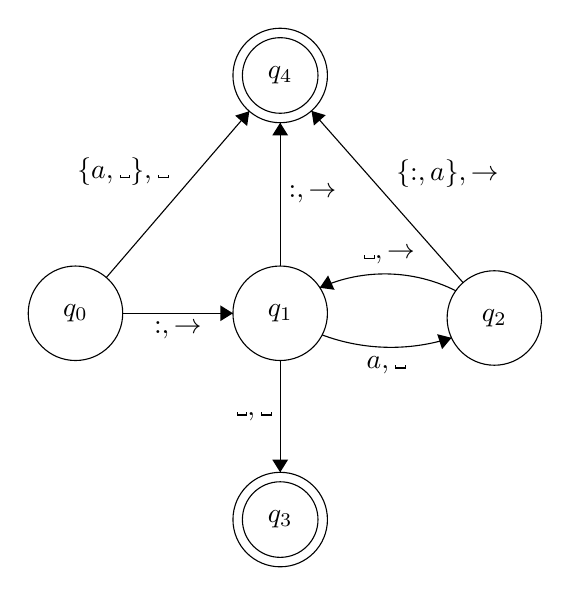
\begin{tikzpicture}[scale=0.2]
\tikzstyle{every node}+=[inner sep=0pt]
\draw [black] (9.4,-31.3) circle (3);
\draw (9.4,-31.3) node {$q_0$};
\draw [black] (22.4,-31.3) circle (3);
\draw (22.4,-31.3) node {$q_1$};
\draw [black] (36,-31.6) circle (3);
\draw (36,-31.6) node {$q_2$};
\draw [black] (22.4,-44.4) circle (3);
\draw (22.4,-44.4) node {$q_3$};
\draw [black] (22.4,-44.4) circle (2.4);
\draw [black] (22.4,-16.2) circle (3);
\draw (22.4,-16.2) node {$q_4$};
\draw [black] (22.4,-16.2) circle (2.4);
\draw [black] (12.4,-31.3) -- (19.4,-31.3);
\fill [black] (19.4,-31.3) -- (18.6,-30.8) -- (18.6,-31.8);
\draw (15.9,-31.8) node [below] {$:,\ra$};
\draw [black] (11.36,-29.03) -- (20.44,-18.47);
\fill [black] (20.44,-18.47) -- (19.54,-18.75) -- (20.3,-19.41);
\draw (15.35,-22.3) node [left] {$\{a,\tvs\},\tvs$};
\draw [black] (33.284,-32.856) arc (-72.05443:-110.47292:12.503);
\fill [black] (33.28,-32.86) -- (32.37,-32.63) -- (32.68,-33.58);
\draw (29.13,-34.02) node [below] {$a,\tvs$};
\draw [black] (24.914,-29.684) arc (114.19527:63.27739:10.059);
\fill [black] (24.91,-29.68) -- (25.85,-29.81) -- (25.44,-28.9);
\draw (29.29,-28.23) node [above] {$\tvs,\ra$};
\draw [black] (22.4,-34.3) -- (22.4,-41.4);
\fill [black] (22.4,-41.4) -- (22.9,-40.6) -- (21.9,-40.6);
\draw (21.9,-37.85) node [left] {$\tvs,\tvs$};
\draw [black] (34.01,-29.35) -- (24.39,-18.45);
\fill [black] (24.39,-18.45) -- (24.54,-19.38) -- (25.29,-18.72);
\draw (29.74,-22.45) node [right] {$\{:,a\},\ra$};
\draw [black] (22.4,-28.3) -- (22.4,-19.2);
\fill [black] (22.4,-19.2) -- (21.9,-20) -- (22.9,-20);
\draw (22.9,-23.75) node [right] {$:,\ra$};
\end{tikzpicture}
\end{center}

What does $T$ do? 

\end{Q}
\begin{comment}
\textbf{Solution}
$T$ erases its input.
\end{comment}

\begin{Q}\label{\prefix Q:delta}
Write out the transition function $\delta$ for $T$ from question \ref{Q:T} in terms of tuples (i.e. $(q,\sigma,q',\sigma'))$.
\end{Q}
\begin{comment}
\textbf{Solution}
\begin{itemize}
\item $(q_0, :, q_1, \ra) = (q_0,\sigma_0,q_1,\sigma_3)$.
\item $(q_0, \tvs, q_4, \tvs) = (q_0,\sigma_1,q_4,\sigma_1)$.
\item $(q_0,a,q_4,\tvs) = (q_0, \sigma_4,q_4,\sigma_1)$.
\item $(q_1, :, q_4, \ra)= (q_1,\sigma_0,q_4,\sigma_3)$.
\item $(q_1,\tvs,q_3,\tvs) = (q_1,\sigma_1,q_3,\sigma_1)$.
\item $(q_1,a,q_2,\tvs) = (q_1,\sigma_4,q_2,\sigma_1)$.
\item $(q_2,:,q_4,\ra) = (q_2,\sigma_0,q_4,\sigma_3)$.
\item $(q_2,\tvs,q_1,\ra) = (q_2,\sigma_1,q_1,\sigma_3)$.
\item $(q_2,a,q_4,\ra) = (q_2,\sigma_4, q_4,\sigma_3)$.
\end{itemize}
\end{comment}

\begin{Q}
Let $T$ be as in question \ref{Q:T}. Using the encoding system from the notes we map every symbol from the alphabet of $T$ to some symbol in $\{\sigma_0,\sigma_1,\ldots\}$. Since $\sigma_0$, $\sigma_1$, $\sigma_2$, and $\sigma_3$ are taken by $:$, $\tvs$, $\la$ and $\ra$ respectively we let $a=\sigma_4$. Using the system from the notes and your transition function from question \ref{Q:delta} write down $\co(T)$.
\end{Q}
\begin{comment}
\textbf{Solution}\\
Assuming tuples in the same order as in the solution above (which is essentially arbitrary - if we were designing a real encoding scheme we would want to use something more principled than this):\\
 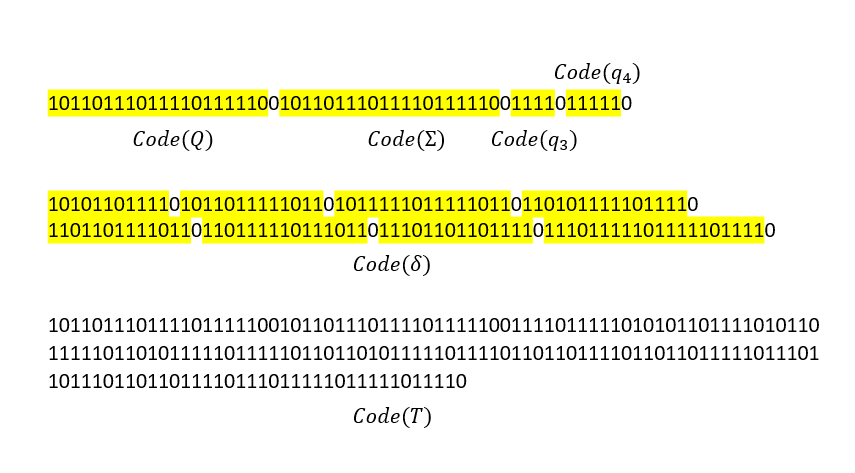
\includegraphics[width=\linewidth]{code.png}
\end{comment}

\begin{Q}
Suppose $T$ is a Turing machine over the alphabet $\{0,1,*\}$ that takes as input two binary numbers separated by $*$ and outputs their sum (in binary). Describe a way we could use $T$ to construct a Turing machine that takes as input two positive binary numbers separated by $*$ and outputs their product. You can use multiple tapes. You don't need to draw a state change diagram.
\end{Q}
\begin{comment}
\textbf{Solution}\\
\begin{enumerate}
\item Copy first number to tape 2.
\item Copy second number to tape 3. 
\item Trim tape 1 so it just contains first number.
\item If tape 3 is empty then erase tape 1 and halt.
\item If the number on tape 3 is one then halt.
\item Add number on tape 2 to the number on tape 1, then decrease number on tape 3 by one (we use $T$ in this step).
\item Go to step 5).
\end{enumerate}

We can assume we have an extra tape for side calculations if we like. We could also check to see if the first number is zero before step 6. Otherwise the machine may add zero to itself several times. This will get the right answer, but is obviously inefficient. 
\end{comment}



\end{document}